\documentclass[a4paper,10pt]{article}
\usepackage[utf8]{inputenc}
\usepackage[spanish]{babel}
\usepackage{hyperref}
\usepackage[pdftex]{graphicx}
\usepackage{amsfonts}
\usepackage{amsmath}

\hypersetup{
  pdftitle={TP1A: Procesamiento de Imágenes - Organización del Computador II},
  colorlinks,
  citecolor=black,
  filecolor=black,
  linkcolor=black,
  urlcolor=black 
}



%opening
\makeatletter

\def\materia#1{\def\Materia{#1}}
\def\tptit#1{\def\tptit{#1}}
\def\res#1{\def\res{#1}} %variable res
\def\integrantes#1{\def\integrantes{ {\sffamily {\fontsize{10pt}{0pt} #1} }} }

\def\keyvar#1{\def\keyvar{#1}}

\newcommand{\Res}[1]{
  
  \begin{abstract}
   \vspace*{-1mm}
  #1
  \end{abstract}
    
}

\newcommand{\keywords}[1]{
\begin{center}
{\footnotesize \textbf{Keywords}
\vskip 4pt
#1

}
\end{center}
}

\renewcommand{\maketitle}{\begin{titlepage}%
      \vspace*{-100pt} % me copa que quede más arriba
     \let\footnotesize\small
    \let\footnoterule\relax
    \parindent \z@
    \reset@font
    \null\vfil
    
\vskip 10\p@
    \hbox{\mbox{%
        \hspace{3pt}%
        \fbox{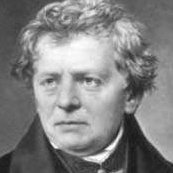
\includegraphics[width=3em]{ohm.jpg}}% IMAGEN LOCA
        \hspace{4pt}
        }
      \vrule depth 0.9\textheight
      \mbox{\hspace{2em}}
            \vtop{% %%%%%%%%%%%%%%%%%%
        \vskip 30\p@
		  \begin{flushleft}
      {\sffamily {\huge \tptit}}
    \end{flushleft}
    \par
    \hrule height 4pt
    \par
    \begin{flushright}
      %\LARGE \Materia \par
     
    {\fontsize{10pt}{0pt} {\sffamily J. Enríquez - LU 36/08 - juanenriquez@gmail.com \par N. Gleichgerrcht - 160/08 - nicog89@gmail.com \par M. Semelman 143/08 - marianosoy@gmail.com}} \par %se pueden poner los autores
     
  
\end{flushright}
    \vskip 30\p@
\Res{\res} % Abstract, pone lo que hay en la variable 'res'
      \vskip 10\p@
  \keywords{\keyvar} % keywords!


\vfill
\vspace*{0mm}
%%%%%%%%%%%%%%%%%%%%%    
 \begin{minipage}[t]{\textwidth}
        \begin{minipage}[t]{.55 \textwidth}
            
\includegraphics{logo_uba.jpg}
        \end{minipage}%%
	 \hspace*{-7mm}
        \begin{minipage}[b]{.55 \textwidth}
            \small{\textbf{\textsf{Facultad de Ciencias Exactas y Naturales}}} \\
            \textsf{Universidad de Buenos Aires} \\
            {\scriptsize %
            %Ciudad Universitaria - (Pabell\'on I/Planta Baja) \\ %% le sacaria el Planta baja y agregaría Depto de computación
              Ciudad Universitaria - (Pabell\'on I) \\  
	      Intendente G\"uiraldes 2160 - C1428EGA \\
            Ciudad Aut\'onoma de Buenos Aires - Rep. Argentina \\
                Tel/Fax: (54 11) 4576-3359 \\
            %http://www.fcen.uba.ar \\ %%corregiría la URL
            http://exactas.uba.ar \\ %%corregiría la URL
	    }
        \end{minipage}
    \end{minipage}%
%%%%%%%%%%%%%%%%%%%%%%
%    \vfil
        }}
%\vfil
%\null
 
  \end{titlepage}%
  \setcounter{footnote}{0}%
}




\makeatother
%\title{Juan Martín Enríquez}
%\author{Tengo un pato}
\tptit{TP2: Redes Eléctricas}
\res{
En este trabajo nos proponemos implementar en lenguaje ensamblador, y usando la arquitectura básica de la IA-32, la detección de bordes en imágenes usando convolución. La técnica consiste en detectar las regiones de la imagen en las que la intensidad cambia abruptamente y graficar esos saltos en nuevas imágenes. \\
\indent Describimos aquí las cuestiones surgidas durante la planificación del algoritmo y su implementación, tarea en la que el énfasis estuvo puesto en maximizar la eficiencia temporal. Además compararemos esa eficiencia con la de una implementación de la biblioteca de procesamiento de imágenes OpenCV y analizaremos las conclusiones surgidas de esa comparación. } % resumen!

\materia{Métodos Numéricos}
\keyvar{Detección Bordes - ASM - Sobel} % palabras claves



\begin{document}

\maketitle
\tableofcontents
\setlength{\parskip}{0.2cm}
\newpage

\section{Introducción}

En la primera entrega de este trabajo hicimos un programa que toma imágenes como
entrada y genera nuevas imágenes efectuando sobre la primera un proceso conocido
como \emph{convolución}. La convolución es una técnica de detección de bordes, y
el resultado es una imagen oscura del mismo tamaño que la original, con zonas
claras donde la imagen fuente tiene ``saltos de intesidad''.

La detección de bordes en imágenes es una técnica utilizada tanto para compresión
de archivos como para lograr efectos gráficos. La convolución consiste en recorrer
los pixeles de la imagen (en nuestro caso en escala de grises) y aplicar en cada
punto un operador de derivación, que es una matriz de números cuyo producto
interno con el entorno del punto mide la variación de la intensidad en alguna
dirección.

Existen muchas matrices utilizadas para la convolución, con diferentes
dimensiones y coeficientes. En la primera entrega nuestro trabajo fue realizar
implementaciones de convolución para las matrices de Roberts (de 2x2), y de
Prewitt y Sobel (de 3x3). La implementación fue realizada en assembler, para la
arquitectura IA-32 básica, es decir usando los registros de propósito general.

Para esta segunda y última parte la tarea consiste en realizar nuevas 
implementaciones aprovechando las nuevas tecnología SIMD: las extensiones MMX,
SSE, SSE2 y SSE3.

Estas extensiones se fueron agregando a los procesadores Intel de forma gradual
(y en ese orden), por lo que algunas computadoras pueden no soportarlas todas.
Todas ellas consisten en sets de instrucciones y hardware especializados para el
procesamiento en paralelo. Los 8 registros \textbf{MMX} de 64 bits y los 8
\textbf{XMM} de 128 bits se comportan como vectores de varios datos (``empaquetados'')
que pueden operarse ``verticalmente'', es decir que entre dos registros se realiza
cada operación elemento a elemento.

Esta tecnología es especialmente útil cuando se necesitan realizar cálculos
sencillos (pues disponemos de pocos registros) de manera repetitiva a lo largo 
de grandes cantidades de datos ``alineados''. Esto es ideal (y está pensado para)
el tratamiento de señales digitales como imágenes y sonidos.

En esta segunda parte rehicimos las implementaciones del primer trabajo y
agregamos una nueva: el operador de Frei-chen, que requiere a diferencia de los
otros un procesamiento en punto flotante. En todos los casos lo hicimos con los
8 registros XMM presentes desde la extensión SSE.

A continuación describiremos el trabajo realizado sin profundizar en las
cuestiones ya analizadas en la parte anterior, sino enfocándonos principalmente
en el nuevo mundo del cálculo en paralelo.




\newpage

\section{Desarrollo}

\subsection{Programa}

El programa que hicimos permite aplicar ciertos operadores de derivación a una imagen especificada por línea de comandos. Los operadores implementados son Roberts, Prewitt y Sobel. El primero tiene matrices de 2x2 y detecta bordes en diagonal. Los otros dos tienen matrices de 3x3 y detectan bordes verticales u horizontales.


%
%acá pondría las matrices de Roberts, Prewitt y Sobel
%


Para cada operador solicitado, aplica la matriz correspondiente en X, luego en Y, y finalmente suma los resultados. Para el caso de Sobel, permite aplicar convolución en una única dirección (X o Y).

%resaltar cvLoadImage y OpenCV
La imagen de entrada puede tener cualquier formato que la función cvLoadImage de OpenCV soporte; todos los formatos comunes están incluidos. Por cada operador utilizado se guarda una nueva imagen en escala de grises (con un sufijo en el nombre que indica el operador y la misma extensión y tamaño que la imagen de entrada) que grafica los bordes detectados.

Por último, el programa muestra por salida estádar la cantidad aproximada de clocks utilizada para la ejecución del algoritmo.

%poner OpenCV y cvSobel en cursiva o algo así
Las implementaciones están hechas en lenguaje ensamblador, aunque el programa también permite usar la implementación del operador Sobel de la biblioteca OpenCV (función cvSobel), así como también grabar la versión en escala de grises de la imagen de entrada. Por último, realiza también detección de bordes usando una primera implementación del operador de Sobel que hicimos en C para ayudarnos a desarrollar el algoritmo y probar variantes.

Para cada punto de la imagen fuente el programa aplica la matriz correspondiente en X, satura el valor a 0 y 255, luego aplica la matriz en Y, satura también su resultado, y finalmente suma ambos coeficientes y satura la suma. Ese valor es grabado en la imagen generada.

Además de la función cvSobel Usamos OpenCV para cargar y guardar imágenes en archivos y transformar imágenes a escala de grises.


\subsection{Algoritmos}
Si bien se trata de procedimientos bastante sencillos e intuitivos, hubo varios aspectos en los que surgieron dudas, problemas o diversidad de posibilidades.

En un píxel en donde la intensidad de la imagen crece hacia la derecha, diremos que se trata de un borde "hacia la derecha". Si en ese punto la imagen en cambio oscurece hacia la derecha, diremos que es un borde "hacia la izquierda".

Notar que, en el caso de Prewitt o Sobel, la matriz de convolución en X (que detecta bordes verticales) arroja un resultado positivo en los bordes hacia la derecha y negativo en los bordes hacia la izquierda. Asimismo la matriz de convolución en Y (que detecta bordes horizontales) produce números positivos en bordes hacia abajo y negativos en bordes hacia arriba. Con las matrices de Roberts pasa lo mismo, salvo que los bordes son positivos hacia el noroeste para la matriz X o hacia el noreste para la Y, y negativos hacia el sudeste o sudoeste respectivamente.

%destacar dx, dy
Hay muchas formas de tratar los valores númerico de la derivación en X y en Y de cada píxel para graficarlos. Con la implementación que hicimos en C de Sobel probamos varias de ellas. Llamaremos dx y dy a los valores obtenidos aplicando derivación en X y en Y.

Una opción es graficar un punto cuya intensidad refleje el módulo del vector (dx, dy). De esta manera se obtiene una imagen oscura con los puntos borde más claros. La imagen muestra los bordes en todas las direcciones, aunque no permite distinguir en qué sentido van. Es decir, un borde hacia la derecha se grafica igual que uno hacia la izquierda. Para el cálculo del módulo puede usarse la norma 2 o bien la norma 1, bastante más rápida de computar.

Otra transformación típica es saturar los valores a un mínimo y a un máximo, lo que permite visualizar los bordes a grandes rasgos sin importar todos los matices de variación. Por ejemplo se los puede saturar a 0 y a 255. Hay que notar que haciendo esto se desprecian todos los bordes negativos, por lo tanto sólo se grafican los bordes que van en un sentido. Si en cambio se suma 128 al valor antes de saturarlo, se puede generar una imagen en la que predomina el gris y donde los bordes positivos se muestran como zonas claras y los bordes negativos como zonas oscuras.

Las variantes que implementamos nosotros son las siguientes:
%esto es una lista
    1) norma 1 de (dx, dy) saturada a 255
    2) dx + dy + 128 saturado a 0 y a 255
    3) saturación de dx y dy a 0 y 255, suma, y saturación de la suma a 255

La idea inicial que teníamos, sugerida en la consigna del trabajo, era implementar la variante 1, que grafica bordes en cualquier dirección. Finalmente, sin embargo, decidimos usar la tercera variante, ya que sus resultados coinciden con los arrojados por la implementación de Sobel de OpenCV, contra la cual deseábamos comparar performance. Esto quiere decir que las imágenes generadas por nuestro programa son oscuras con zonas claras donde la imagen original tiene aumentos de intensidad hacia abajo o hacia la derecha (hacia el noroeste o hacia el noreste en el caso de Roberts). Los bordes que van en sentido contrario no se reflejan de ninguna manera así que es imposible saber dónde están o cuán abruptos son.

La variante 2 produce gráficos diferentes e interesantes de observar. Se pueden ver bordes en ambos sentidos, graficados de manera distinta. Los bordes positivos en blanco y los negativos en negro. Sin embargo no muestra bordes en todas las direcciones. De hecho, el efecto de sumar la derivada en X con la de Y es que los bordes se grafican en una única dirección (una diagonal). Los bordes perpendiculares a esta diagonal hacen que dx se anule con dy y por lo tanto no se visualizan.

En el momento que optamos sumar las derivadas en X y en Y porque la técnica usada por OpenCV parecía ser esa, surgió una idea: en lugar de aplicar la matriz de X, luego la de Y y sumar los resultados, sería más eficiente (y más sencillo de implementar) hacer una sola pasada usando la matriz suma de las dos matrices. Esto razonamiento es, además de intuitivo, matemáticamente correcto.

Sin embargo las imágenes generadas aún no eran iguales a las de OpenCV. Algunos bordes, pese a ser "positivos", estaban ocultos. Lo que sucede es que por ejemplo una derivada positiva en X se puede anular con una derivada negativa en Y. Esto hace que se vean casi exclusivamente los bordes que apuntan en dirección sudeste.

Finalmente se concluyó que la técnica correcta (para generar dibujos como los de OpenCV) era saturar cada derivada parcial a 0 y a 255 y recién después sumarlas. Como la primera saturación elimina negativos, es imposible que las derivadas se cancelen, y se visualizan todos bordes que apuntan hacia abajo y/o hacia la derecha.


\subsection{Implementación}

%%algo sobre el bug de unsigned char

%%algo sobre los bugs de assembler

%%algo sobre push/pop vs. registros




\newpage

\section{Resultados}


\newpage

\section{Discusión}

%destacar rdtsc
Tratándose de implementaciones en lenguaje en ensamblador, uno de las cuestiones que más tuvimos en cuenta y analizamos fue, por supuesto, la eficiencia de los algoritmos. Como ya dijimos, lo que hicimos fue medir la cantidad de clocks de procesador que cada función (incluso la de OpenCV y la que escribimos en C) consumen. Esto se logró mediante invocaciones desde C a la función \texttt{rdtsc} de lenguaje ensamblador.

El resultado que obtuvimos en ese sentido fue, como esperábamos, que nuestras implementaciones en ensamblador no alcanzaron la rapidez de la implementación de OpenCV, y que la implementación hecha en C fue aún más lenta. Los siguientes gráficos reflejan estas diferencias para imágenes de distintos tamaños.\footnote{\emph{ Las ejecuciones fueron realizadas en una PC: MSI Wind U100 con procesador Intel Atom N270 - 1Gb de RAM y bajo el S.O. Ubuntu Netbook Remix 9.04}}

%%

%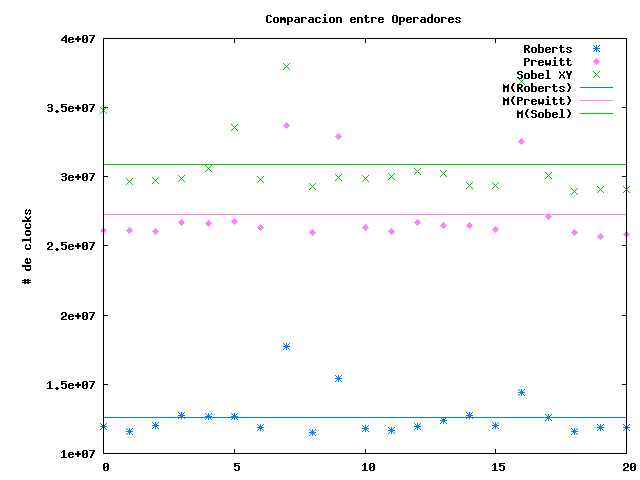
\includegraphics[scale=0.5]{graf1.png}

\medskip

\begin{center}
\begin{tabular}{lrrr}
\cr  & Roberts & Prewitt & Sobel\\
\hline
\emph {Media} & 12618185 & 27276745 & 30886607 \\
\emph {Desvío} & 1511854 & 2448652 & 2598392\\
\emph {Max} & 17743236 & 33694296 & 37954836\\
\emph {Min} & 11549460 & 25707576 & 28905552\\
\hline \\
\end{tabular}
\end{center}



%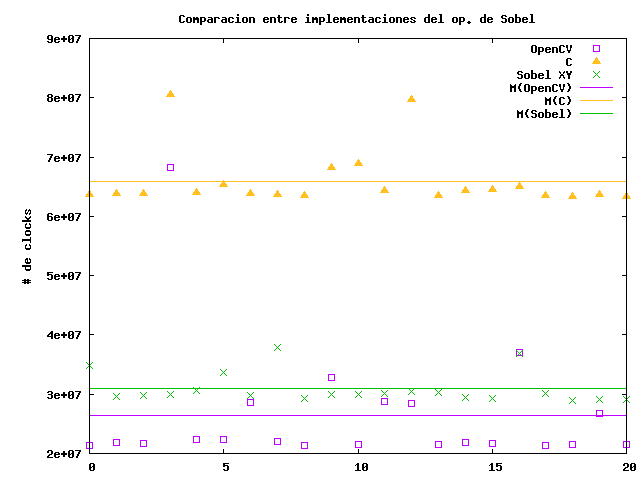
\includegraphics[scale=0.5]{sobels.png}

\medskip

\begin{center}
\begin{tabular}{lrrr}
\cr  & OpenCV & C & ASM \\
\hline
\emph {Media} & 26412756 & 65944312 & 30886607 \\
\emph {Desvío} & 10563470 & 4921205 & 2598392\\
\emph {Max} & 68276028 & 80518500 & 37954836\\
\emph {Min} & 21301152 & 63370956 & 28905552\\
\hline \\
\end{tabular}
\end{center}



%%

La diferencia de eficiencia entre la implementación en C y las hechas en ensamblador tiene un motivo claro y conocido. Por naturaleza, los lenguajes de programación de más alto nivel nos abstraen de muchas cuestiones de implementación, pero a la vez nos quitan control sobre esa implementación. Mientras en ensamblador usamos directamente los registros del procesador (memoria más rápida de la máquina) en C éstos se usan de manera interna y el programador trabaja con datos en memoria RAM.

Esta razón bastaría para justificar las diferencias de rendimiento, pero no es la única: además, el sólo hecho de estar programando en un lenguaje de nivel superior hace que el programador ponga menos atención en los detalles de eficiencia y más en otros aspectos como la legibilidad del código o su reutilizabilidad.

En cambio, el motivo de la diferencia de rendimiento entre nuestras implementaciones en ensamblador y la de OpenCV resulta menos evidente. De hecho no estudiamos el código que utiliza OpenCV. Sabemos, sin embargo, que nuestras implementaciones no aprovechan al máximo las posibilidades de los procesadores, a diferencia de las de OpenCV que seguramente utilizan capacidades más avanzadas y/o específicas de los mismos como por ejemplo el uso de MMX, SSE, etc..

Un ejemplo que se nos ocurre es la saturación: nosotros, para cada píxel, verificamos si el resultado está por debajo de 0 o por encima de 255 para ajustarlo. Estos chequeos y ajustes consumen un tiempo significativo de ejecución; es claro que usando aritmética saturada nativa del procesador se mejoraría mucho la performance.

Otra característica que imaginamos se podría aprovechar es la paralelización: al tratarse de cálculos sencillos y repetitivos podrían venir bien las instrucciones de datos empaquetados.

También resulta interesante observar en qué medida se aceleró el algoritmo cuando eliminamos los accesos a memoria innecesarios que realizábamos al utilizar la pila en lugar de sólo los registros. El gráfico que sigue compara el rendimiento de la primera implementación en ensamblador que hicimos (que aplicaba Roberts en X usando la pila) con la definitiva (que minimiza los accesos a memoria y aplica Roberts en ambas direcciones). Es notorio que, aunque la primera implementación realiza menos cálculos pues aplica una sola matriz en lugar de dos, sea tanto menos eficiente por no aprovechar al máximo los registros del procesador.

%%

%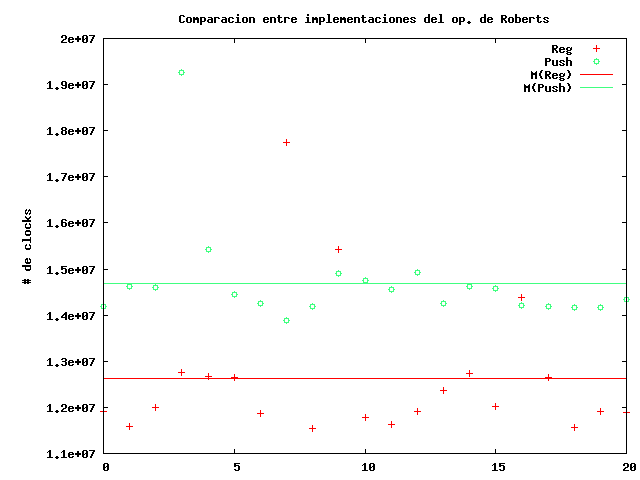
\includegraphics[scale=0.5]{roberts.png}

\medskip

\begin{center}
\begin{tabular}{lrr}
\cr  & ``Reg'' & ``Push''  \\
\hline
\emph {Media} & 12618185 & 14692721  \\
\emph {Desvío} & 1511854 & 1105330 \\
\emph {Max} & 68276028 & 19269852 \\
\emph {Min} & 11549460 & 13878600 \\
\hline \\
\end{tabular}
\end{center}

%%


\newpage

\section{Conclusiones}

Con la realización del presente trabajo pudimos apreciar la mejora que se tiene
al implementar un algoritmo con instrucciones del tipo SIMD.
De acuerdo a la experimentación realizada, pudimos observar que esta mejora consiste
en una eficiencia aproximadamente 10 veces más grande.

Si bien los resultados obtenidos son óptimos es evidente la limitación que en 
principio tienen estas instrucciones ya que como se dijo en la introducción, no 
todos los algoritmos son paralelizables al estilo SIMD. Sin embargo y como se
notó en este trabajo, son ideales para el procesamiento de imágenes.
Pareciera que toda transformación que se quiere aplicar a imágenes (o a sonidos)
encontrará en SIMD una herramienta poderosa.

Como ya dijimos, pese a la relativa simplicidad con la que se pueden llevar a
cabo este tipo de algoritmos en esta arquitectura, queremos mencionar nuevamente
que esto requiere un esfuerzo adicional, y en muchos casos trabas importantes.
Además, el código resultante es mucho menos declarativo, así como también mucho
más sensible a cambios.

Por último queremos observar que no hay motivo para conformarse con los registros
\textbf{XMM}. De la misma manera, nuevas arquitecturas podrían proveer no 8 sino
16 o 32 registros, no de 128 bits sino de 256 o 1024. En ese caso se manifestará
la poca reusabilidad de la paralelización, pues las implementaciones hechas para
8 registros de 128 bits claramente no van a aprovechar los nuevos 16 o 32 registros.

A priori podría pensarse en un esquema en el que el código no esté tan atado a
cómo acomodar los datos, sino que tenga sentido en diferentes arquitecturas de
cálculo en paralelo, aprovechando en cada caso la cantidad provista de registros
y bits. Para ello haría falta trabajar con código de más alto nivel, pensando en
qué operaciones se deben paralelizar pero no de a cuántas. Las cuestiones de 
acomodamiento de datos quedaría en manos de un compilador. Es una posibilidad
muy complicada pero también muy interesante, y sólo con el paso del tiempo 
conoceremos su factibilidad.


\newpage

%\input{bib.tex}

\bibliographystyle{acm}
\bibliography{biblio.bib}
\end{document}
